\documentclass[frenchb, paper=a4, fontsize=11pt]{scrartcl}

\usepackage[utf8x]{inputenc}
\usepackage[T1]{fontenc}
\usepackage{lmodern}

\usepackage{ifthen}
\usepackage{url}


\usepackage{multirow}

% Color
% cfr http://en.wikibooks.org/wiki/LaTeX/Colors
\usepackage{color}
\usepackage[usenames,dvipsnames,svgnames,table]{xcolor}
\definecolor{dkgreen}{rgb}{0.25,0.7,0.35}
\definecolor{dkred}{rgb}{0.7,0,0}

\newcommand{\matlab}{\textsc{Matlab}}

% Math symbols
\usepackage{amsmath}
\usepackage{amssymb}
\usepackage{amsthm}
\DeclareMathOperator*{\argmin}{arg\,min}
\DeclareMathOperator*{\argmax}{arg\,max}


% Sets
\newcommand{\Z}{\mathbb{Z}}
\newcommand{\R}{\mathbb{R}}
\newcommand{\Rn}{\R^n}
\newcommand{\Rnn}{\R^{n \times n}}
\newcommand{\C}{\mathbb{C}}
\newcommand{\K}{\mathbb{K}}
\newcommand{\Kn}{\K^n}
\newcommand{\Knn}{\K^{n \times n}}

% Unit vectors
\usepackage{esint}
\usepackage{esvect}
\newcommand{\kmath}{k}
\newcommand{\xunit}{\hat{\imath}}
\newcommand{\yunit}{\hat{\jmath}}
\newcommand{\zunit}{\hat{\kmath}}
\newcommand{\uunit}{\hat{\umath}}

% rot & div & grad & lap
\DeclareMathOperator{\newdiv}{div}
\newcommand{\divn}[1]{\nabla \cdot #1}
\newcommand{\rotn}[1]{\nabla \times #1}
\newcommand{\grad}[1]{\nabla #1}
\newcommand{\gradn}[1]{\nabla #1}
\newcommand{\lap}[1]{\nabla^2 #1}


% Elec
\newcommand{\B}{\vec B}
\newcommand{\E}{\vec E}
\newcommand{\EMF}{\mathcal{E}}
\newcommand{\perm}{\varepsilon} % permittivity

\newcommand{\bigoh}{\mathcal{O}}
\newcommand\eqdef{\triangleq}

\DeclareMathOperator{\newdiff}{d} % use \dif instead
\newcommand{\dif}{\newdiff\!}
\newcommand{\fpart}[2]{\frac{\partial #1}{\partial #2}}
\newcommand{\ffpart}[2]{\frac{\partial^2 #1}{\partial #2^2}}
\newcommand{\fdpart}[3]{\frac{\partial^2 #1}{\partial #2\partial #3}}
\newcommand{\fdif}[2]{\frac{\dif #1}{\dif #2}}
\newcommand{\ffdif}[2]{\frac{\dif^2 #1}{\dif #2^2}}
\newcommand{\constant}{\ensuremath{\mathrm{cst}}}

\usepackage{siunitx}

\usepackage{tikz}
\usepackage{tikz-3dplot}

\usepackage{pgfplots}
\usepackage{lmodern}
%\usepackage[protrusion=true,expansion=true]{microtype}
\usepackage{xspace}

\usepackage{babel}
% Listing
% always put it after babel
% http://tex.stackexchange.com/questions/100717/code-in-lstlisting-breaks-document-compile-error
\usepackage{listings}

\definecolor{mygreen}{rgb}{0,0.6,0}
\definecolor{mygray}{rgb}{0.5,0.5,0.5}
\definecolor{mymauve}{rgb}{0.58,0,0.82}
\lstset{ %
  language=Matlab,
  backgroundcolor=\color{white},   % choose the background color; you must add \usepackage{color} or \usepackage{xcolor}
  basicstyle=\footnotesize,        % the size of the fonts that are used for the code
  breakatwhitespace=false,         % sets if automatic breaks should only happen at whitespace
  breaklines=true,                 % sets automatic line breaking
  captionpos=b,                    % sets the caption-position to bottom
  commentstyle=\color{mygreen},    % comment style
  deletekeywords={...},            % if you want to delete keywords from the given language
  escapeinside={\%*}{*)},          % if you want to add LaTeX within your code
  extendedchars=true,              % lets you use non-ASCII characters; for 8-bits encodings only, does not work with UTF-8
  frame=single,	                   % adds a frame around the code
  keepspaces=true,                 % keeps spaces in text, useful for keeping indentation of code (possibly needs columns=flexible)
  keywordstyle=\color{blue},       % keyword style
  otherkeywords={*,...},           % if you want to add more keywords to the set
  numbers=none,                    % where to put the line-numbers; possible values are (none, left, right)
  numbersep=5pt,                   % how far the line-numbers are from the code
  numberstyle=\tiny\color{mygray}, % the style that is used for the line-numbers
  rulecolor=\color{black},         % if not set, the frame-color may be changed on line-breaks within not-black text (e.g. comments (green here))
  showspaces=false,                % show spaces everywhere adding particular underscores; it overrides 'showstringspaces'
  showstringspaces=false,          % underline spaces within strings only
  showtabs=false,                  % show tabs within strings adding particular underscores
  stepnumber=2,                    % the step between two line-numbers. If it's 1, each line will be numbered
  stringstyle=\color{mymauve},     % string literal style
  tabsize=2,	                   % sets default tabsize to 2 spaces
  title=\lstname                   % show the filename of files included with \lstinputlisting; also try caption instead of title
}

\KOMAoptions{DIV=last}

\usepackage[top = 2.5 cm, bottom = 3 cm, left = 2.5 cm, right = 2.5 cm]{geometry}
\usepackage{hyperref}
\usepackage{todonotes}
\usepackage[makeroom]{cancel}

%%% Custom sectioning (sectsty package)
\usepackage{sectsty}								% Custom sectioning (see below)
\allsectionsfont{\scshape}						% Change font of al section commands

%%% Custom headers/footers (fancyhdr package)
\usepackage{fancyhdr}
\pagestyle{fancyplain}
\fancyhead{}										% No page header
\fancyfoot[L]{\small Groupe 1}					% You may remove/edit this line 
\fancyfoot[C]{}									% Empty
\fancyfoot[R]{\thepage}							% Pagenumbering
\renewcommand{\headrulewidth}{0pt}				% Remove header underlines
\renewcommand{\footrulewidth}{0pt}				% Remove footer underlines
\setlength{\headheight}{13.6pt}
\newcommand*\eq[1]{\overline{#1}} 				% equilibre


%%% Equation and float numbering
\numberwithin{equation}{section}					% Equationnumbering: section.eq#
\numberwithin{figure}{section}					% Figurenumbering: section.fig#
\numberwithin{table}{section}						% Tablenumbering: section.tab#

%%% Maketitle metadata
\newcommand{\horrule}[1]{\rule{\linewidth}{#1}} 	% Horizontal rule

\title{
		%\vspace{-1in} 	
		\usefont{OT1}{bch}{b}{n}
		\normalfont \normalsize \textsc{Ecole polytechnique de Louvain} \\ [25pt]
		\horrule{0.5pt} \\[0.4cm]
		\large LINMA1510 - Automatique linéaire\\
		\huge Laboratoire 1 - Contrôle du niveau d'eau dans un réservoir \\
		\horrule{1.5pt} \\[0.5cm]
}
\author{
		\normalfont
		\textsc{Groupe 62}\\
      	Antoine Paris\hspace{0.6cm} Philippe Verbist \\	
       	\normalsize
        \today
}
\date{}

\begin{document}
\maketitle

\section*{TO DO}

\begin{itemize}
\item refaire les mesures avec les KP, KI mesurés
\end{itemize}


\section{Modèle et données}

Le modèle repose sur les équations suivantes:
\begin{itemize}
\item équation de continuité:
\begin{equation}
\frac{dh_3}{dt} = \frac{1}{S_R}q_{P3} - \frac{1}{S_R}(q_{F30}+q_{S30})
\label{eq:contnuity}
\end{equation}
\item loi de Toricelli:
\begin{align}
q_{F30}& = S_{F30} \sqrt{2gh_3} \label{eq:toricelliF}\\
q_{S30} &= S_{S30} \sqrt{2gh_3} \label{eq:toricelliS}.
\end{align}
\end{itemize}

En outre, nous avons les données suivantes
\begin{align}
S_R& = \SI{43}{cm^2}\\
g &= \SI{981}{cm\per\second^2}
\end{align}

\section{Expliquer les valeurs choisies pour $\eq{q}_{P3}$ et $\eq{h}_3$. Expliquer le calcul de la surface $S_{S30}$}

\begin{figure}[!ht]
	\centering
	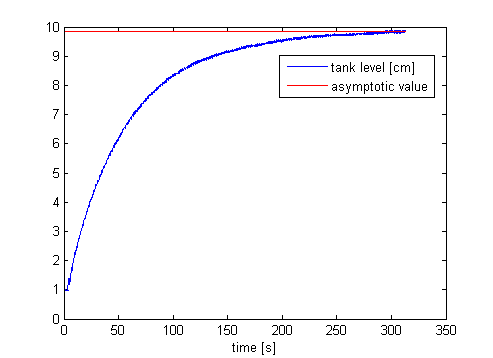
\includegraphics[width=0.6\linewidth]{img/exp1_ol.png}
	\caption{Point d'équilibre du système en boucle ouverte, avec $u_0 = \SI{30}{\milli\liter\per\second}$}
	\label{fig:exp1_ol}
\end{figure}


Lors de l'expérience, la valeur de $q_{P3}$ a été imposée  à $u_0 = \SI{30}{\milli\liter\per\second}$. La hauteur $h_3$ correspond à la valeur d'équilibre lorsque la valve frontale $S_{F30}$ est fermée et la valve $S_{S30}$ ouverte (voir la figure \ref{fig:exp1_ol}). Leur valeur chiffrée vaut
\begin{align}
q_{P3} & = \SI{30}{[\milli\liter\per\second]}\\
h_3 & = \SI{10.1}{[cm]}.
\end{align}

Nous avons travaillé dans les mêmes conditions expérimentales pour calculer $S_{S30}$ ($q_{F30} = 0$ et $\frac{dh_3}{dt} = 0$). Ainsi, à l'équilibre, en reprenant les équations \ref{eq:contnuity} et \ref{eq:toricelliS}, nous avons
\begin{align}
&\cancel{\frac{dh_3}{dt}} = \frac{1}{S_R}\eq{q}_{P3} - \frac{1}{S_R}(\cancel{q_{F30}}+q_{S30})\\
\Leftrightarrow & \eq{q}_{P3} = S_{S30} \sqrt{2g\eq{h}_3} \\
\Leftrightarrow & S_{S30} = \frac{\eq{q}_{P3}}{ \sqrt{2g\eq{h}_3}} = \SI{0.21}{cm^2}
\end{align}

\section{Détailler le calcul du modèle linéarisé et le calcul des fonctions de transfert $G(s)$ and $H(s)$}

\subsection{Calcul du modèle linéarisé}

Soit le système initial
\begin{align}
x &= h_3 \\
u &= q_{P3}\\
v &= S_{F30}\\
\end{align}
Régit par les équations
\begin{align}
\frac{dx}{dt} &= f(x,u,v) = \frac{1}{S_R}u - \frac{1}{S_R}(v\sqrt{2gx} + S_{S30}\sqrt{2gx})\\
y &= h(x,u,v) = x
\end{align}
Pour linéariser ce système, on procède au changements de variables
\begin{align}
\chi &= x-\eq{x} = x - 9.84\\
\rho &= u-\eq{u} = u - 30\\
\nu &= v - \eq{v} = v\\
\phi &= y - h(\eq{x}) = y - 30\\
\end{align}
et on réécrit le système sous la forme
\begin{equation}
\left\{ \begin{array}{ccc}
\frac{d\chi}{dt} &=& A\chi + B\rho \\
\phi &=& C\chi + D\rho
\end{array}
\right.
\end{equation}

avec 
\begin{align}
A& = \frac{\partial f(x,u,v)}{\partial x}\rvert_{(\eq{x},\eq{u},\eq{v})} = -\frac{1}{S_R}(v\frac{g}{\sqrt{2gx}} + S_{S30}\frac{g}{\sqrt{2gx}})\rvert_{(\eq{x},\eq{u},\eq{v})} \\
&= -\frac{1}{S_R	} S_{S30} \frac{g}{\sqrt{2g\eq{x}}} = \SI{-.0345}{\per\second}\\
B &=\left[ \begin{array}{l}
 \frac{\partial f}{\partial u}\rvert_{\eq{x}} \\
  \frac{\partial f}{\partial v} \rvert_{\eq{x}}\\
\end{array} \right] 
= \left[ \begin{array}{l}
 \frac{1}{S_R} = \SI{0.0233}{cm\per \milli\liter}\\
  \frac{\sqrt{2g\eq{x}}}{S_R}= \SI{-3.27}{cm \per\milli\liter}\\
\end{array} \right] \\
C &= \frac{\partial h}{\partial x}\rvert_{\eq{x}} = \SI{1}{cm/cm}\\
D&=\left[ \begin{array}{l}
 \frac{\partial h}{\partial u}\rvert_{\eq{x}} \\
  \frac{\partial h}{\partial v} \rvert_{\eq{x}}\\
\end{array} \right]  = \left[ \begin{array}{l}
0\\
0
\end{array} \right] \SI{}{cm s \per mL}
\end{align}
\todo{Vérifier les unités}

\subsection{Calcul des fonctions de transfert}
\begin{align}
G(s) &= C(sI-A)^{-1}B_u + D = \frac{B_u}{s-A}= \frac{0.02326}{s+0.03454}\\
H(s) &= C(sI-A)^{-1}B_v + D = \frac{B_v}{s-A} = \frac{-3.274}{s+0.03454}\\
\end{align}

Remarquons que l'on peut calculer la constante de temps du système (puisque $G(s) = \frac{B/A}{1-s/A}$)
\begin{equation}
\tau_{OL} = -\frac{1}{A} \approx \SI{29}{s}
\end{equation}

\section{Fonctions de transfert en boucle fermée}

Nous considérons maintenant un contrôleur PI tel que représenté à la figure \ref{fig:closed_loop}.

\begin{figure}[!ht]
	\centering
	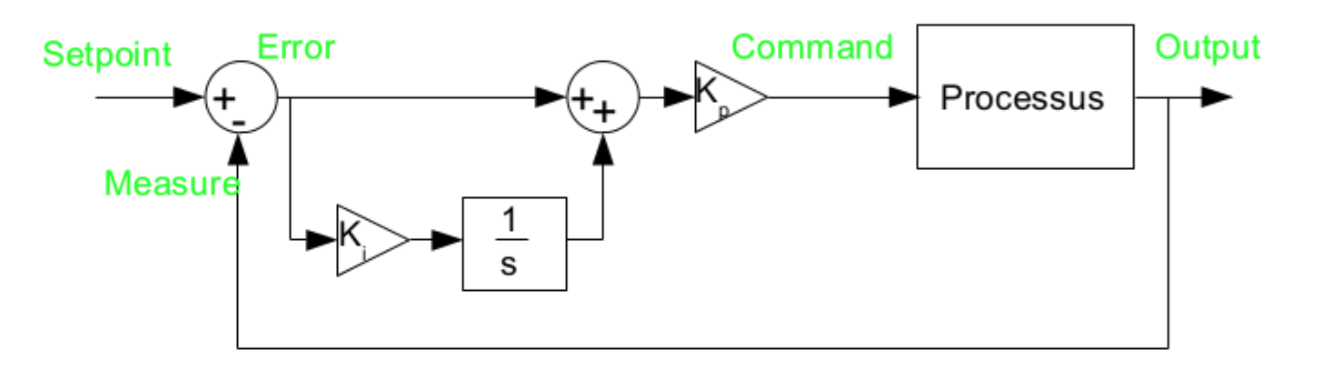
\includegraphics[width=\linewidth]{img/closed_loop.png}
	\caption{Diagramme de bloc du système contrôlé par un contrôleur PI}
	\label{fig:closed_loop}
\end{figure}


On trouve
\begin{align}
T_r(s) & \triangleq \frac{y}{r}\rvert_{v=0}\\
y &= K_P G \left(e+\frac{eK_I}{s} \right)\\
& = K_P G\left(r-y+\frac{(r-y)K_I}{s} \right)\\
y(s-A) & = K_P B_u\left( r(1+\frac{K_I}{s}) - y(1+\frac{K_I}{s})\right)\\
y(s-A + B_uK_P + \frac{B_uK_P K_I}{s}) & = B_uK_P  \ r \left(1+\frac{K_I}{s} \right) \\
y(s^2 +(B_uK_P-A)s + B_uK_P K_I) & = B_uK_P  \ r \left(s+K_I \right) \\
\frac{y}{r}&= \frac{B_uK_P  (s+K_I )}{s^2 +(B_uK_P-A)s + B_u K_P K_I} = T_r(s)
\end{align}

De même,
\begin{align}
T_v(s) & \triangleq \frac{y}{v}\rvert_{r=0}\\
y &= H v+ G K_P (e+\frac{eK_I}{s})\\
&= H v + G K_P(-y-\frac{-yK_I}{s}) \\
y(s-A) &= B_v v - y B_u K_P (1+\frac{K_I}{s})\\
y(s^2 + (B_u K_P-A)s + B_u K_P K_I) &= B_v v s\\
\frac{y}{v} & = \frac{B_v s}{s^2 + (B_u K_P-A)s + B_u K_P K_I} = T_v(s)
\end{align}

Une autre manière (plus facile) pour arriver à ces résultats est de considérer le contrôleur 
\begin{equation}
C(s) = (1+\frac{K_I}{s})K_P = \frac{1}{s}(s+K_I)K_P
\end{equation}
et de calculer ensuite
\begin{align}
T_r(s) &= \frac{C(s)G(s)}{1+C(s)G(s)} = \frac{(s+K_I)K_P B_u}{s(s-A)+(s+K_I)K_P B_u}\\
T_v(s) &= \frac{H(s)}{1+C(s)G(s)} = \frac{B_v s}{s(s-A)+(s+K_I)K_P B_u}
\end{align}

\section{Analyse des performances de différents contrôleurs avec une perturbation}

\begin{figure}[!ht]
\centering
\begin{minipage}{.5\textwidth}
  \centering
  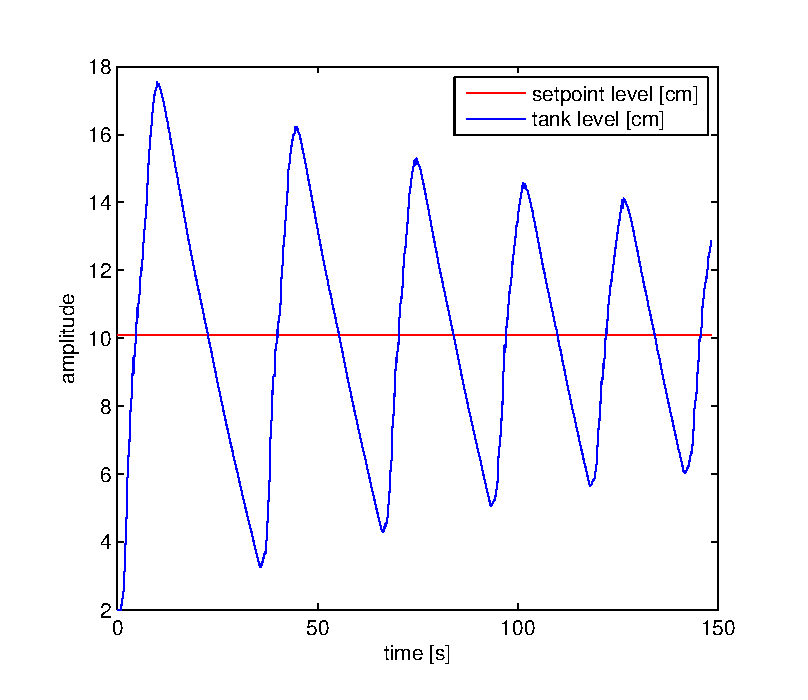
\includegraphics[width=.99\linewidth]{img/cl-2_5-2.eps}
  \captionof{figure}{$\left\{K_P,K_I\right\}=\left\{2.5,2\right\}$}
  \label{fig:test1}
\end{minipage}%
\begin{minipage}{.5\textwidth}
  \centering
  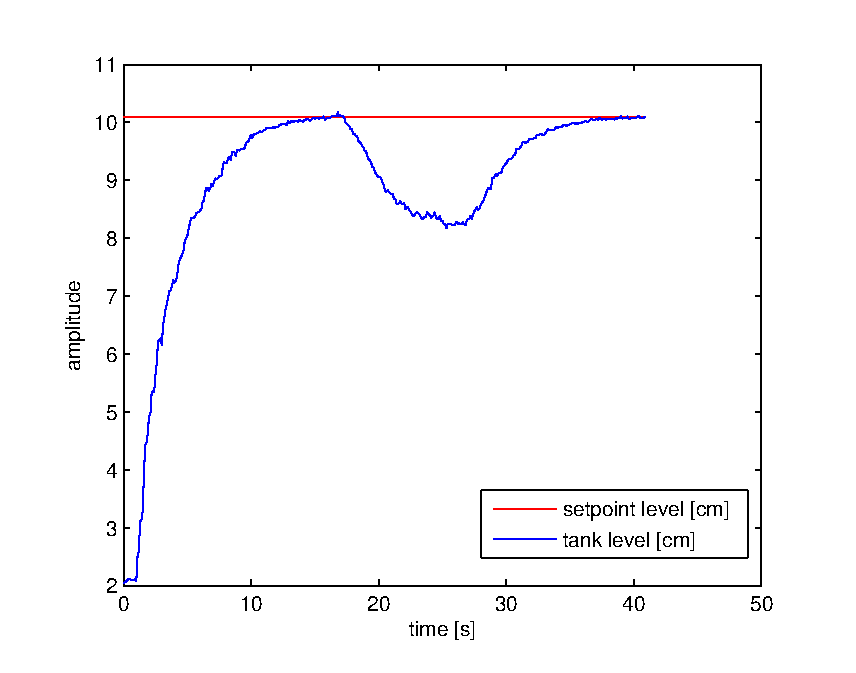
\includegraphics[width=.99\linewidth]{img/cl-10-0.eps}
  \captionof{figure}{$\left\{K_P,K_I\right\}=\left\{10,0\right\}$}
  \label{fig:test2}
\end{minipage}
\end{figure}

\begin{figure}[!ht]
\centering
\begin{minipage}{.5\textwidth}
  \centering
  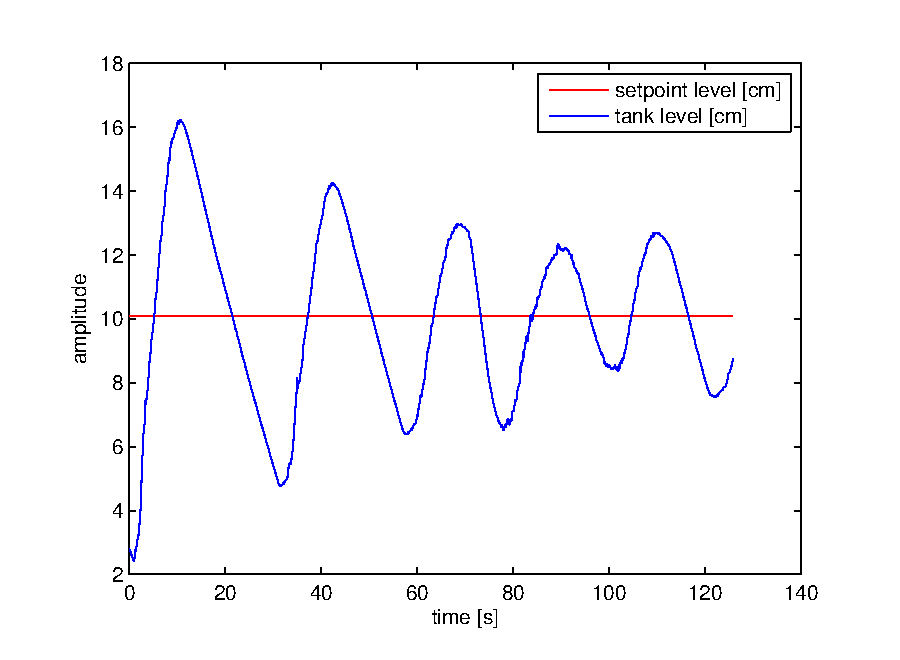
\includegraphics[width=.99\linewidth]{img/cl-3-1.eps}
  \captionof{figure}{$\left\{K_P,K_I\right\}=\left\{3,1\right\}$}
  \label{fig:test3}
\end{minipage}%
\begin{minipage}{.5\textwidth}
  \centering
  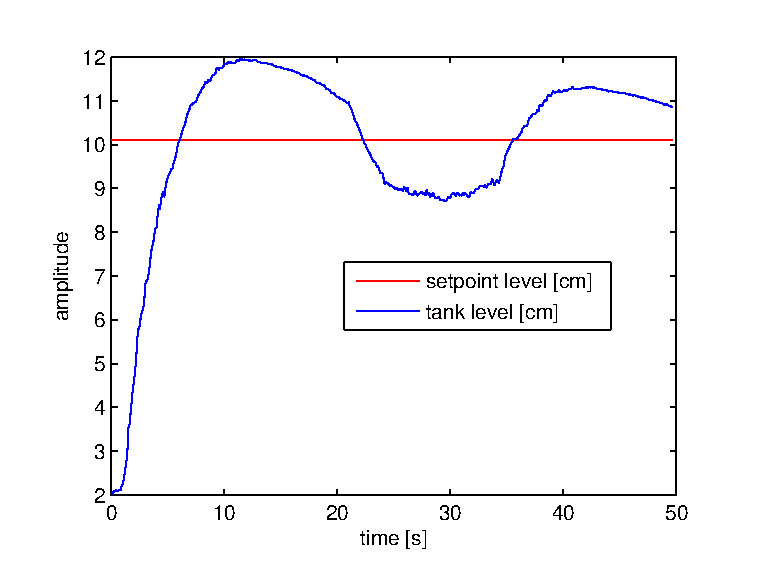
\includegraphics[width=.99\linewidth]{img/cl-10-0_1.eps}
  \captionof{figure}{$\left\{K_P,K_I\right\}=\left\{10,0.1\right\}$}
  \label{fig:test4}
\end{minipage}
\end{figure}





\section{Calcul des paramètres $K_P,K_I$ pour satisfaire certaines spécifications}

\subsection{Sans simplification}
Les spécifications sont:
\begin{itemize}
\item pas d'overshoot
\item un temps de réponse trois fois plus petit que le système naturel (non contrôlé)
\end{itemize}
Reprenons le dénominateur de la fonction de transfert $G_{CL}(s)$:
\begin{equation}
D(s) = s^2 +(B_u K_P -A)s + B_u K_P K_I
\end{equation}
que nous pouvons reprocher de la forme canonique suivante pour un système du deuxième ordre
\begin{equation}
D_c(s) = s^2 + 2\zeta \omega_n s + \omega_n^2.
\end{equation}
Par identification, on obtient
\begin{align}
\omega_n &= \sqrt{B_u K_P K_I} \label{eq:ns_omegan}\\
\zeta &= \frac{B_u K_P-A}{2\sqrt{B_u K_P K_I}}
\end{align}
Les spécifications nous imposent:
\begin{align}
\zeta &\ge 1\\
\tau & = \frac{1}{\omega_n(\zeta - \sqrt{\zeta^2-1})} = \frac{\tau_{OL}}{3}\approx \SI{10}{s} \label{eq:ns_tau}
\end{align}
En imposant $\zeta = 1.5$, et en résolvant les équations \ref{eq:ns_omegan} à \ref{eq:ns_tau}, on trouve
\begin{align}
K_P &= 18.97\\
K_I &= 0.0891
\end{align}
La présence d'un zéro dans la fonction de transfert fait apparaitre un overshoot qu'il nest pas possible de contrôler de manière canonique. 
La comparaison théorie/résultats se trouvce à la figure \ref{fig:final_values_1}.


\subsection{Avec simplification pôle-zéro}
En posant 
\begin{equation}
K_I = -A
\end{equation}
on obtient une simplification pôle-zéro, et la fonction de transfert devient
\begin{equation}
T_r(s) = \frac{K_P B_u}{s+K_P B_u}= \frac{1}{1+\frac{s}{K_P B_u}}.
\end{equation}

S'agissant d'une fonction du premier ordre, il n'y a pas de dépassement, et le temps de réponse vaut 
\begin{equation}
\tau = \frac{1}{K_P B_u} = \frac{\tau_{OL}}{3} 
\end{equation}

On trouve les valeurs chiffrées suivantes
\begin{align}
K_P &= 4.55\\
K_I &= 0.035
\end{align}
La comparaison théorie/résultats se trouvce à la figure \ref{fig:final_values_2}.

\begin{figure}[!ht]
	\centering
	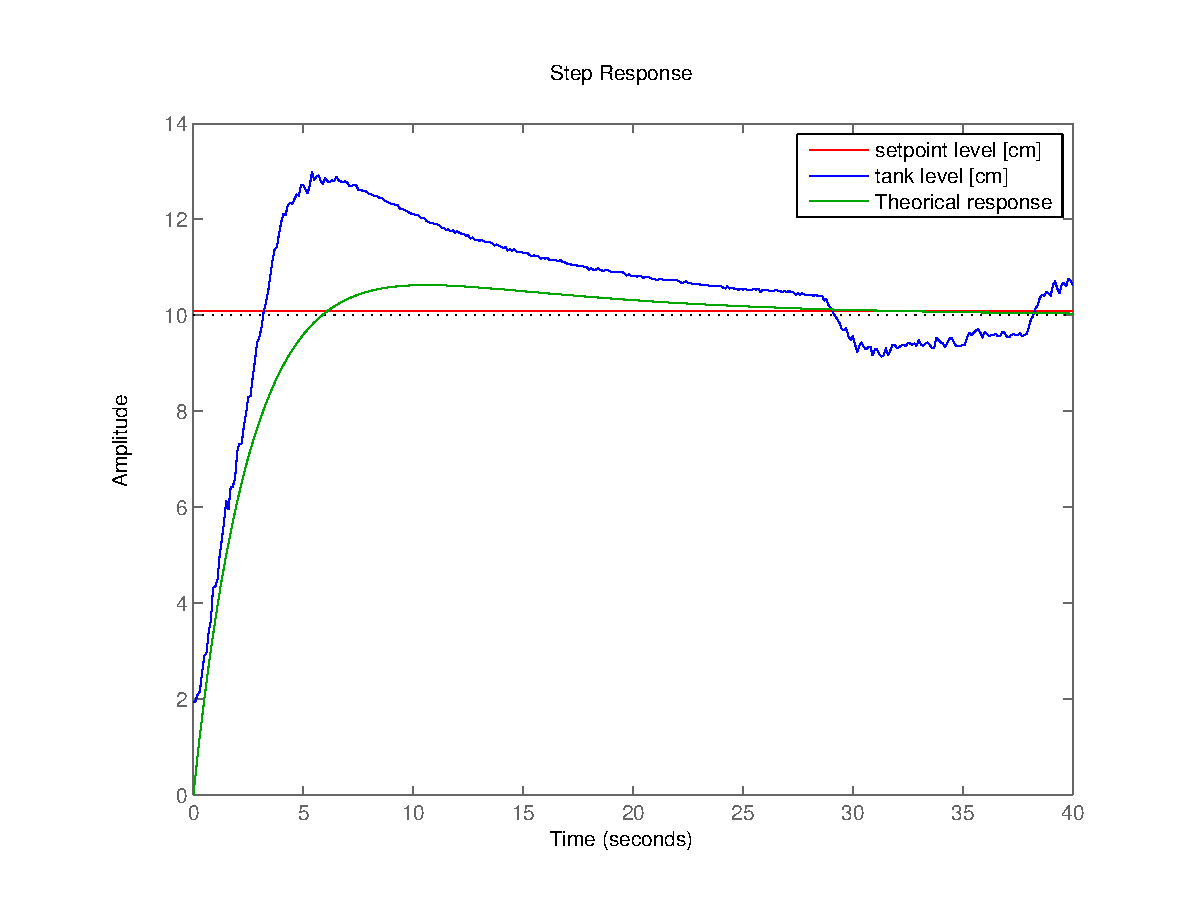
\includegraphics[width=0.8\linewidth]{img/cl_ultimate_without_simplification.eps}
	\caption{Réponse du système avec $\left\{K_P,K_I \right \} = \left\{18.97,0.089\right\}$}
	\label{fig:final_values_1}
\end{figure}

\begin{figure}[!ht]
	\centering
	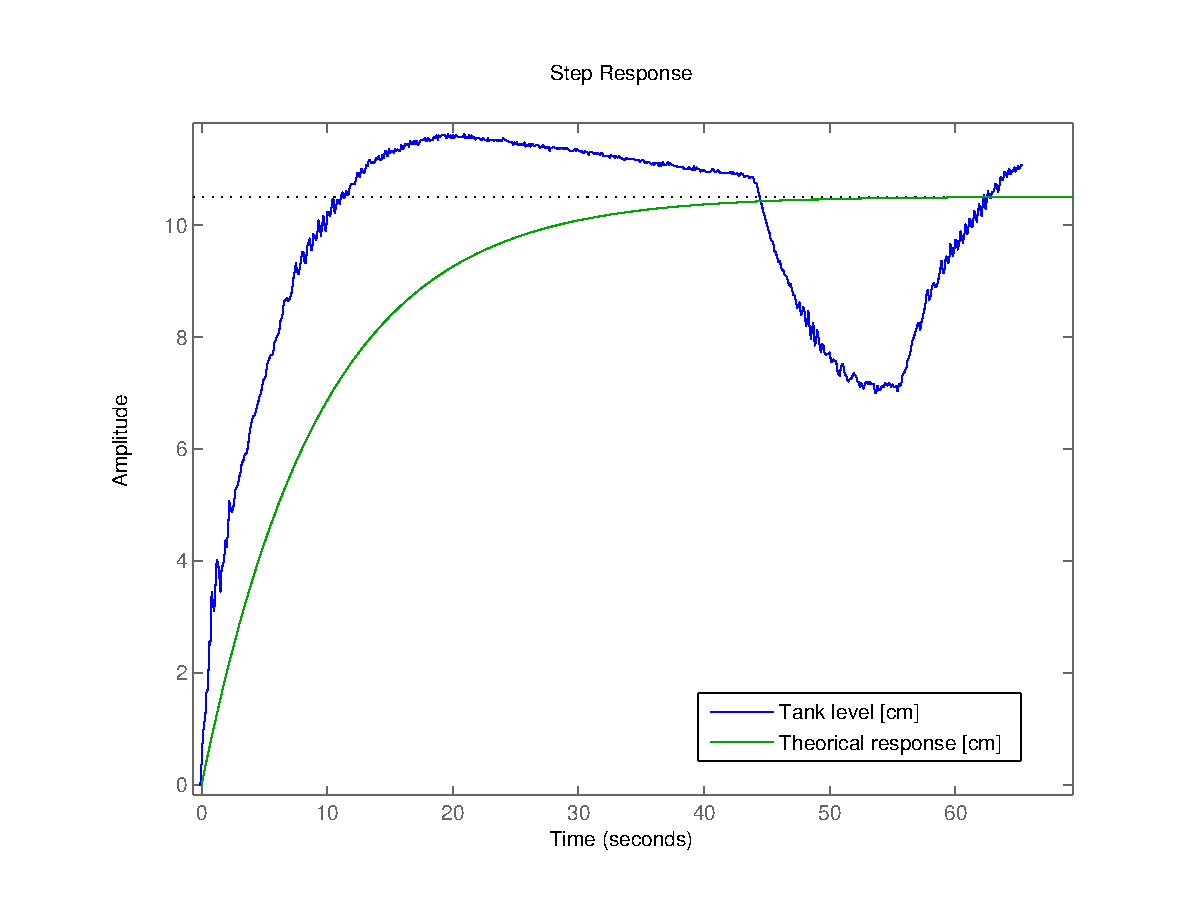
\includegraphics[width=0.8\linewidth]{img/cl_ultimate.eps}
	\caption{Réponse du système avec $\left\{K_P,K_I \right \} = \left\{4.55,0.035\right\}$}
	\label{fig:final_values_2}
\end{figure}


\section{Non-linéarités du système contrôlé}
La non-linéarité principale vient du fait que le système d'équations initiales n'est pas linéaire, et qu'il a dû être linéarisé autour de son point d'équilibre. Ainsi, lorsque l'on ne se trouve pas proche de ce point d'équilibre, les équations que nous avons ne sont pas correctes.














\end{document}